\documentclass{article} 
\usepackage[utf8]{inputenc}
\usepackage[T2A]{fontenc}
\usepackage[russian, english]{babel}
\usepackage{graphicx}	
\usepackage{amsmath, amssymb}
\usepackage{titlesec}
\newcommand\tab[1][1cm]{\hspace*{#1}}
\usepackage[14pt]{extsizes}
\usepackage{setspace,amsmath}
\usepackage[left=20mm, top=15mm, right=15mm, bottom=15mm, nohead, footskip=10mm]{geometry} 
\usepackage{mathtext}
\usepackage[dvipsnames]{xcolor}
\usepackage{ragged2e}
\sloppy
\usepackage{caption}
%--------------------------------------------------------------------
\begin{document}                                                         
\newpage
\thispagestyle{empty}

\begin{center}
Федеральное государственное образовательное бюджетное учреждение\\ высшего профессионального образования\\ 
\textbf{«Финансовый университет при Правительстве Российской Федерации»}\\
\end{center}
	
\vspace{2em}
	
\begin{center}
\textbf{Департамент анализа данных, принятия решения и финансовых технологий}\\ 
\end{center}
	
\vspace{2em}
	
\begin{center}
\textbf{Курсовая работа\\
\vspace{3mm}}
по дисциплине \textbf{"Технологии анализа данных и машинное обучение"} на тему: \\ \vspace{2em} \textbf{"Разработка и построение рекомендательной системы"}\\
\vspace{3mm}
Вид исследуемых данных: Рейтинг и история просмотра пользователей аниме-сериалов\\
\end{center}
	
\vspace{6em}
		
\begin{flushright}
Выполнила:\\
студентка группы ПМ3-1\\
Баданина Н. Д.\\
Научный руководитель:\\
к.э.н., доцент\\
Гринева Наталья Владимировна
\end{flushright}
	
\vspace{\fill}
	
\begin{center}
Москва 2020
\end{center}

%--------------------------------------------------------------------
\newpage
	
\renewcommand*\contentsname{Содержание}
\makeatletter
\renewcommand{\l@section}{\@dottedtocline{1}{0em}{2em}}
\renewcommand{\l@subsection}{\@dottedtocline{1}{0em}{2.6em}}
\renewcommand{\l@subsubsection}{\@dottedtocline{1}{0em}{3.2em}}

\makeatother
\setcounter{page}{2}

\begin{center}
	\tableofcontents
\end{center}

%--------------------------------------------------------------------
\newpage
\addcontentsline{toc}{section}{Введение}
\begin{center}
	\section*{Введение\vspace{5mm}}
\end{center}
\tabРаньше маркетинг был традиционным. До появления современных технологий продавец в локальном магазине знал о своих покупателей гораздо больше, чем требовалось для продажи. Можно сказать, что предложения продавца покупателю были персонализированными или таргетинговыми. 
С развитием современных технологий и экстенсивным ростом индустрии, большие бизнесы, получающие доход с продаж, уже не знаю своих клиентов лично. В лучшем случае о клиенте известные общая информация, например пол или регион проживания. На этом этапе появляется не персонализированная реклама: баннеры, вывески и т. д. Телевидение, несмотря на свой охват, тоже предлагает не таргетинговую рекламу. Допустим, некоторый канал в определенное время смотрят работающие мужчины, больше информации извлечь невозможно. На основе таких данных рекомендации будут неэффективные: слишком общие или неактуальные. Проблема сбора данных решается с появление сети Интернет. Сейчас о пользователе можно узнать геопозицию, каким телефоном и браузером он пользуется, личные данные и увлечения из профилей социальных сетей. Особенностью сбора данных через интернет является то, что пользователь сам указывает начальную информацию о себе: ФИО, город, номер телефона и т. д.. Остальные данные получают исходя из поведения клиента. 
Однако, и при этом подходе, рекомендации могут быть слабо персонализированными в силу специфичности данных. Сложно сделать вывод о том, что нужно некому Васе, который зашел в мобильное приложение в 13:00. На этом этапе развития появляется машинное обучение, которое, обработав массив данных о пользователе, может сделать неочевидный вывод, что некому Васе можно продать обед.\\
\tabАлгоритмы машинного обучения, которые предсказывают какой фильм/статью/товар/услугу купит пользователей называют рекомендательными системами. В основном такие системы используются для рекомендаций фильмов (Netflix, YouTube), товаров (Яндекс.Маркет, Ozon), музыки (Яндекс.Музыка) и статей (Яндекс.Дзен). 
 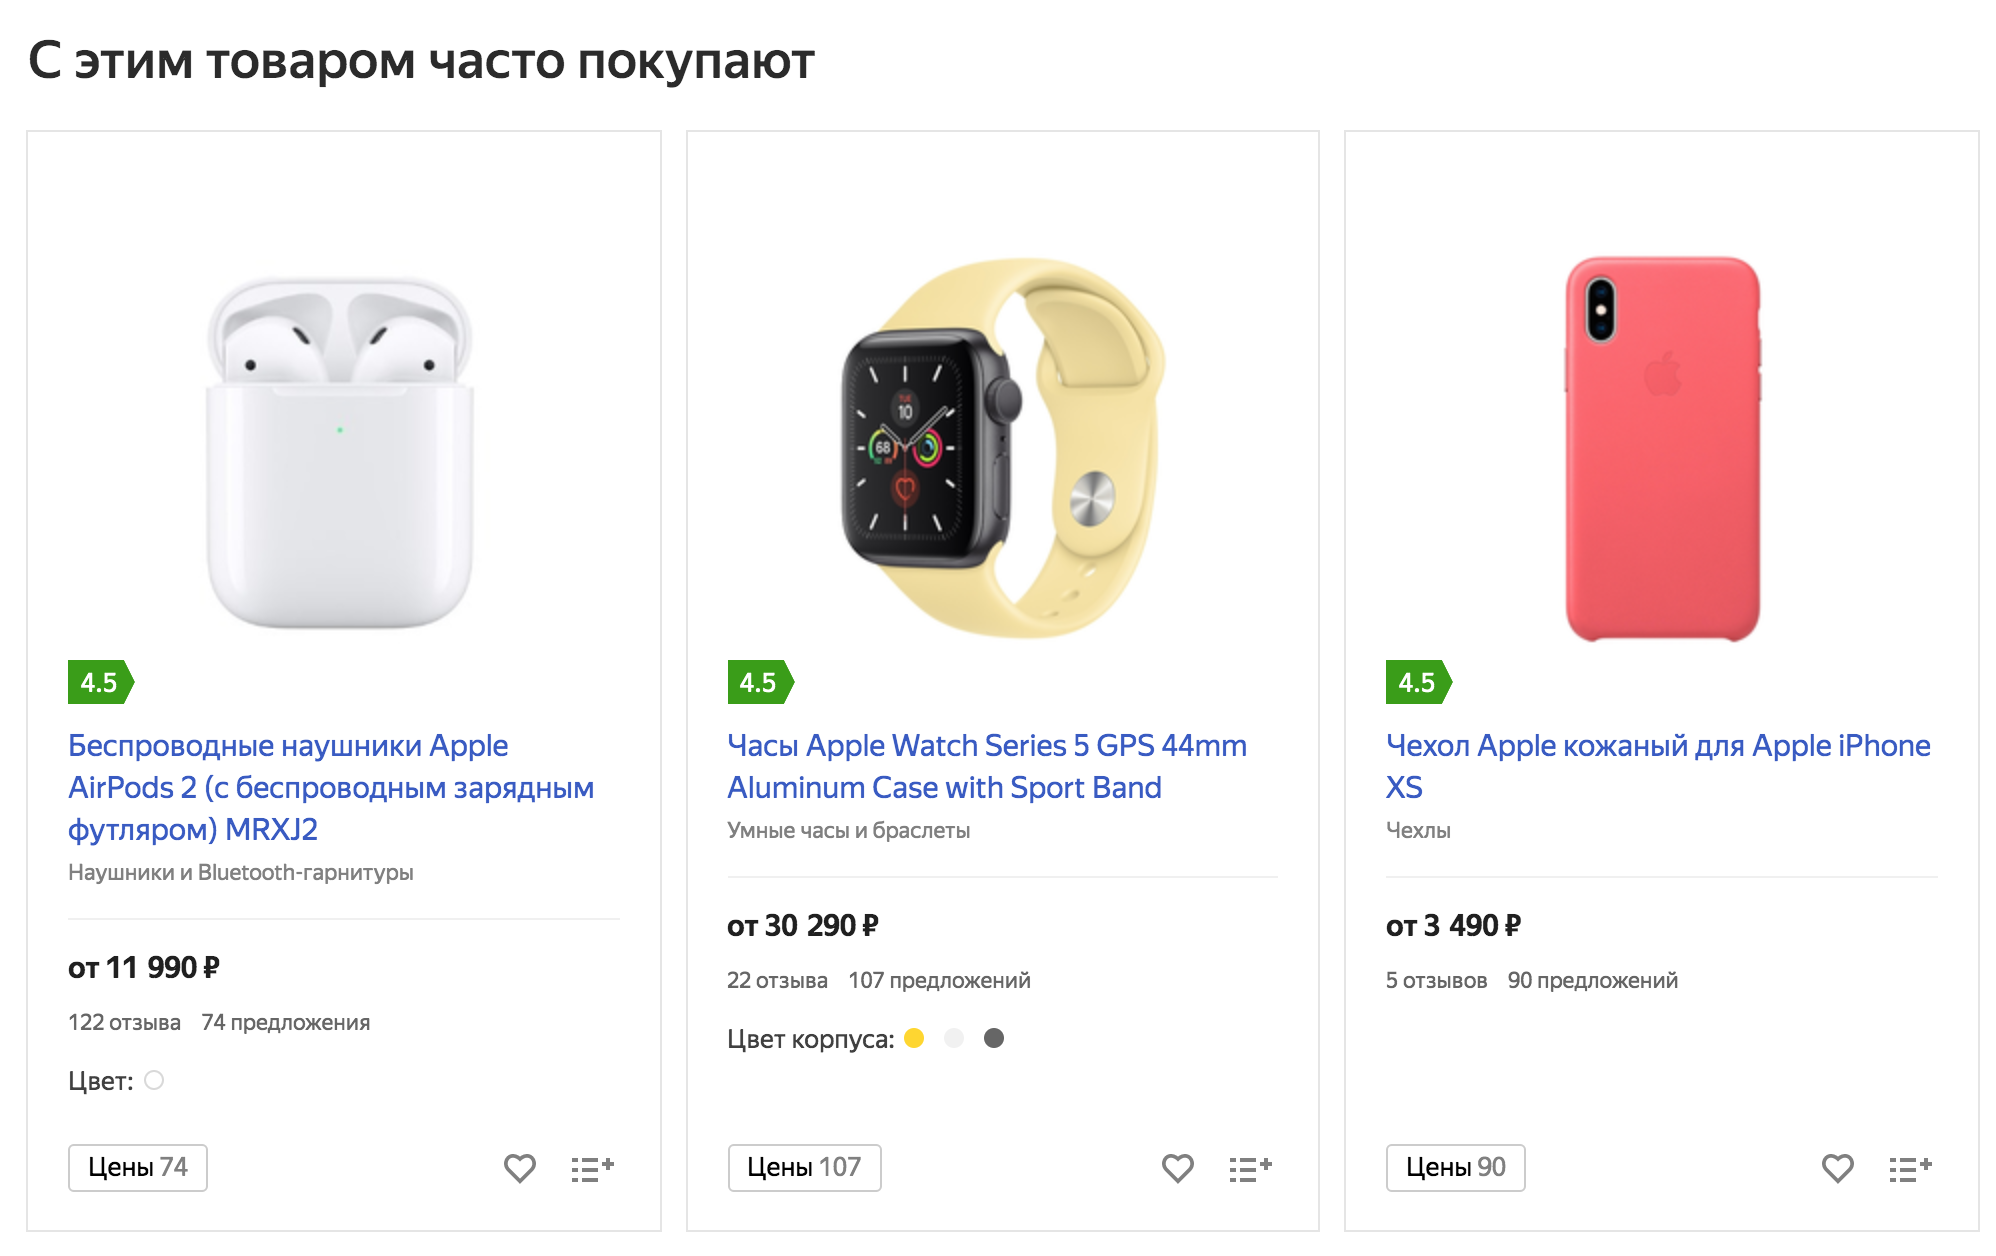
\includegraphics[width=\linewidth]{f1.png}\\
\tabНапример, так выглядят рекомендации к товару Iphone 11 Pro на Яндекс.Маркет. Можно заметить недоработку: рекомендуют купить чехол к другой модели телефона.\\
\tabКлиент получает информацию, а сервис зарабатывает на предоставлении качественных услуг. Услуги — это не обязательно прямые продажи предлагаемого товара. Сервис также может зарабатывать на комиссионных или просто увеличивать лояльность пользователей, которая потом выливается в рекламные и иные доходы. Интересно, что даже страницы в поиске сейчас персонализированы и разным пользователям по одному и тому же запросу могут быть предложены разные ссылки на сайт.\\
\tabВ данной работе рассмотрено построение рекомендательной системы для совета аниме-сериала пользователю. По оценкам McKinsey, $75\%$ выручки онлайн кинотеатра Netflix приходится именно на рекомендованные фильмы/сериалы и процент этот, вероятно, будет расти. Рынок японских анимационных сериалов только развивается в России, поэтому система будет актуальная для многих сервисов, таких как Ivi, Okko и Кинопоиск, которые ещё не внедрили контент этого типа на свои платформы.\\
\qquad 

%--------------------------------------------------------------------
\newpage

\section*{Теоретическая часть}
\tabРекомендательные сервисы многообразны, так как их основные характеристики могут сильно отличаться. Любую рекомендательную систему можно описать с помощью таких характеристик, как \\
\tab– предмет рекомендации: товары (Amazon, Ozon), статьи (Arxiv.org), новости (Surfingbird, Яндекс.Дзен), люди (Linkedin, LonelyPlanet), музыка (Last.fm, Pandora), плейлисты и так далее. В целом, рекомендовать можно что угодно. \\
\tab– цель рекомендации. Зачем рекомендуется: покупка, информирование, обучение, заведение контактов. \\
\tab– контекст рекомендации. Что пользователь в этот момент делает: смотрит товары, слушает музыку, общается с людьми. \\
\tab– источник рекомендации – кто рекомендует: аудитория (средний рейтинг ресторана в TripAdvisor), схожие по интересам пользователи, экспертное сообщество (бывает, когда речь о сложном товаре, таком, как, например, вино).\\
\tab– cтепень персонализации. Неперсональные рекомендации – когда вам рекомендуют то же самое, что всем остальным. Они допускают таргетинг по региону или времени, но не учитывают ваши личные предпочтения. Более продвинутый вариант – когда рекомендации используют данные из вашей текущей сессии. Вы посмотрели несколько товаров, и внизу страницы вам предлагаются похожие. Персональные же рекомендации используют всю доступную информацию о клиенте, в том числе историю его покупок.\\
\tab– прозрачность. Люди больше доверяют рекомендации, если понимают, как именно она была получена. Так меньше риск нарваться на «недобросовестные» системы, продвигающие проплаченный товар или ставящие более дорогие товары выше в рейтинге. Кроме того, хорошая рекомендательная система сама должна уметь бороться с купленными отзывами и накрутками продавцов. Манипуляции бывают и непреднамеренными. Например, когда выходит новый блокбастер, первым делом на него идут фанаты, соответственно, первую пару месяцев рейтинг может быть сильно завышен.\\
\tab– формат рекомендации. Это может быть всплывающее окошко, появляющийся в определенном разделе сайта отсортированный список, лента внизу экрана или так далее.\\
\tab– алгоритмы. К наиболее классическим относятся алгоритмы Summary-based (неперсональные), Content-based (модели основанные на описании товара), Collaborative Filtering (коллаборативная фильтрация), Matrix Factorization (методы основанные на матричном разложении). Некоторые из них были реализованы в практике.
%--------------------------------------------------------------------
\newpage
\subsection*{Постановка задачи\vspace{5mm}}

\tabЗадача рекомендательной системы — найти для пользователя такие элементы из заданного множества, которые с высокой вероятностью ему понравятся. Например: товары, которые пользователь захочет купить; фильмы, которые пользователю понравятся; статьи, которые пользователь дочитает до конца.\\
\tabВведем некоторые стандартные обозначения. Пользователи — множество U (users). В этой работе в множество U попадают пользователи сайта, поставившие какому-либо аниме-сериалу оценку. Новые пользователи рассматриваться не будут, так как возникает проблема "холодного старта", при которой у программы недостаточно информации для рекомендации. Подробно эта проблема будет рассмотрена ниже.\\
\tabТовары — множество I (items). В множестве I это могут быть любые категории товаров: и фильмы, и музыка, и техника. — зависит от задачи. В этой работе в качестве множества I выступает список аниме-сериалов. Так же будем считать, что для некоторой пары пользователь-товар $u\in U$ и $i\in I$ известна оценка $r_{ui}$, выражающая заинтересованность пользователя в этом товаре.\\
\tabЗаинтересованность может выражаться в разных единицах. В случае с музыкой, это может быть, как много раз пользователь слушал данный трек, как много раз дослушал до конца, лайкнул ли он его. В случае со статьями дочитал ли он его до конца, сколько раз кликнул, скорость проматывания страницы и так далее. В данной работе заинтересованность принимает вид рейтинга, находящегося в промежутке от 1 до 10, поставленного пользователем аниме-сериалу. \\
\tabТребуется по известным оценкам заинтересованности научиться находить для каждого пользователя $u$ набор из $k$ товаров $I(u)$, наиболее подходящих пользователю, то есть таких, для которых оценка $r_{ui}$ окажется максимальной. То есть в итоге задача сводится к тому, что для объекта вида $x_{ui}$ надо уметь предсказывать оценку $r_{ui}$. Как и в любой задаче машинного обучения, требуется уточнить три пункта: целевая переменная, признаки, функционал ошибки. Первый пункт был рассмотрен выше. Теперь время перейти к тому, какие признаки характеризуют пару пользователь-товар.

%--------------------------------------------------------------------
\newpage
\section*{Признаки}
\subsection*{Статистические признаки}

\tabДля начала рассмотрим простые типы факторов. Среди них могут быть: количество покупок и просмотров данного товара, количество покупок пользователя в данной категории, количество покупок пользователей.\\
\tabЕсли товар или пользователь уже набрали достаточно статистики, то часто такие признаки оказываются самыми главными при принятии решения, поскольку уже содержат в себе достаточно информации о предпочтениях. Так, используя эти признаки, можно рекомендовать популярные товары в той категории, что нравится пользователю.

%--------------------------------------------------------------------
\subsection*{Коллаборативная фильтрация}

\tabМетоды коллаборативной фильтрации строят рекомендации для пользователя на основе схожести между пользователями и товарами. Различают несколько подходов:\\
\tab— Memory-based\\
\tab— Модели со скрытыми переменными\\
\tab— Гибридный: объединение вышеперечисленных подходов.\\
\tabРассмотрим memory-based подход. В его основе лежит таблица $R$, размерности $N\times M$, где $N$ — количество пользователей, а $M$— количество товаров. Это матрица, по одной из осей которой отложены все клиенты сервиса (Users), а по другой – объекты рекомендации (Items). На пересечении некоторых пар (user, item) данная матрица заполнена оценками (Ratings) – это известный нам показатель заинтересованности пользователя в данном товаре, выраженный по заданной шкале (например от 1 до 10). На пересечении строки $u$ и столбца $i$ хранится значение $r_{ui}$, если оно известно. Здесь стоит отметить, что, в основном, такая матрица будет состоять из нулей или пропусков, так как товаров много, а процент покупок, в отношении к количеству позиций, маленькое. Вытекающим из этого замечания является вывод о том, что в программе необходимо хранить всю матрицу рейтингов, которая имеет большую размерность. Это не только в разы увеличивает время работы, но и усложняет визуализацию и процесс вычислений с использованием этой матрицы. \\
\tabПользователи обычно оценивают лишь небольшую часть товаров и задача рекомендательной системы – обобщить эту информацию и предсказать отношение клиента к другим товарам, про которые ничего не известно. Другими словами нужно заполнить все незаполненные ячейки. Шаблоны потребления у людей разные, и не обязательно должны рекомендоваться новые товары. Можно показывать повторные позиции, например, для пополнения запаса. По этому принципу выделяют две группы товаров: повторяемые и неповторямые, например, книги или фильмы, которые редко приобретают повторно. Выделяя повторяемые товары в категорию можно сократить размерность матрицы $R$.
 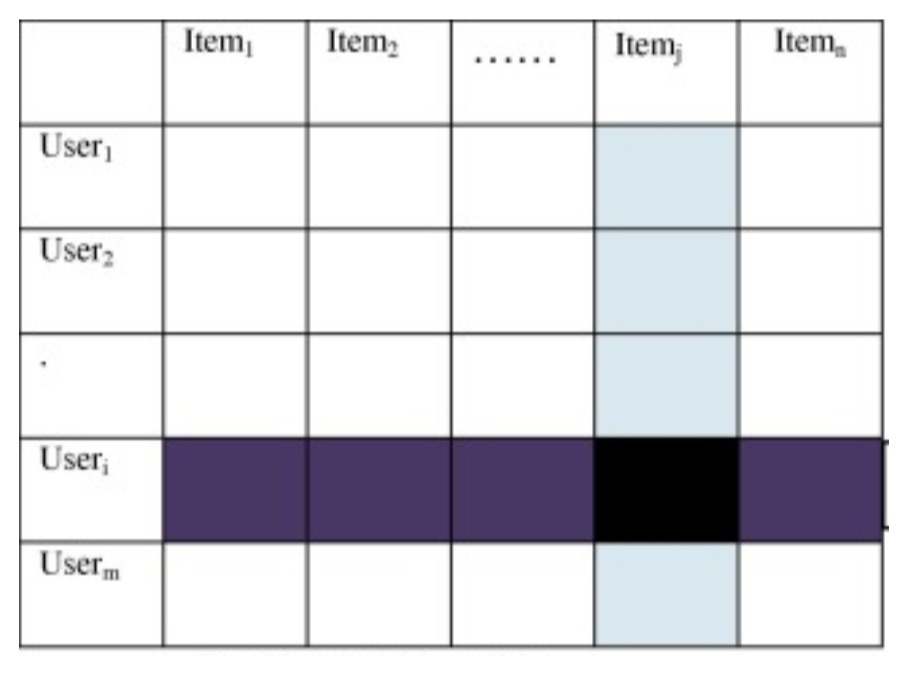
\includegraphics[width=\linewidth]{f2.png}\\
 Матрица $R$.
%--------------------------------------------------------------------
\subsubsection*{Baseline}
\tabСамое простое предсказание, которое можно сделать, имея таблицу $R$, посчитать среднее всех известных оценок и считать, что и остальным товарам пользователи будут ставить именно такие оценки:\\
$\mu=\frac{\sum_U{\sum_I{r_{ui}}}}{|Y|}$, где $Y$ — множество известных оценок.\\ 
\\
\tabНо понятно, что такой подход имеет множество недостатков, и один из них заключается в том, что мы не учитываем предвзятость пользователей и популярность товаров. Для того, чтобы учесть данные характеристики, найдем среднюю оценку для каждого товара и для каждого пользователя:\\
$\mu_i=\frac{\sum_U{r_{ui}}}{n_i}$\\
\vspace{1.5mm}\\
$\mu_u=\frac{\sum_I{r_{ui}}}{m_u}$, где ${n_i}$ и ${m_i}$ — количество оценок у товара $i$ и пользователя $u$ соответственно.\\
\tabПосчитав сдвиги для пользователей и товаров относительно средней оценки, можно более точно вычислить, какую же оценку пользователь $u$ поставит товару $i$:\\
$b_i=\mu_i-\mu$\\
$b_u=\mu_u-\mu$\\
$r_{ui}=\mu+b_i+b_u$\\
\tabНо пока мы никак не учитывали схожесть пользователей. Получается, что при подсчете средней оценки на неё влияли как пользователи со схожими вкусами, так и те, вкусы которых сильно разнятся. Поэтому можем немного модифицировать подсчет среднего: будем считать среднее для всех товаров для выбранного пользователя $u_0$, при этом влияние других пользователей будет зависеть от их схожести с выбранным пользователем:\\
$\mu=\frac{\sum_U{sim(u_0,u)}\sum_I{r_{ui}}}{|Y|}$\\
\vspace{1.5mm}\\
\tabСоответственно так же можно модифицировать подсчет средней оценки для товаров.
%--------------------------------------------------------------------
\subsubsection*{Сравнение пользователей и товаров}
\tabВозникает вопрос: как сравнивать схожесть пользователей. Будем исходить из следующего предположения: два пользователя считаются похожими, если они ставят одним и тем же товарам одинаковые оценки. Рассмотрим двух пользователей $u$ и $v$. Обозначим через $I_{uv}$ множество товаров $i$, для которых известны оценки обоих пользователей:\\
$I_{uv}=\{ i\in I | \exists r_{ui} \& \exists r_{vi}\}$\\
Тогда сходство между двумя данными пользователями можно вычислить с помощью корреляции Пирсона:\\
$sim(u,v)=\frac{\sum_{i\in I_{ui}}{(r_{ui}-\mu_u)(r_{vi}-\mu_v)}}{\sum_{i\in I_{uv}}{(r_{ui}-\mu_u)^2}\sum_{i\in I_{uv}}{(r_{vi}-\mu_u)^2}}$\\
Чтобы вычислить сходство между товарами $i$ и $j$ так же введем множество пользователей $U_{ij}$, для которых известны оценки для этих товаров.\\
$U_{uj}=\{u\in U|\exists r_{ui} \&\exists r_{uj}\}$\\
Тогда сходство двух товаров можно вычислить через корреляцию Пирсона:\\
$sim(i,j)=\frac{\sum_{u\in U_{ij}}{(r_{ui}-\mu_i)(r_{uj}-\mu_j)}}{\sum_{u\in U_{ij}}{(r_{ui}-\mu_i)^2}\sum_{u\in U_{ij}}{(r_{ui}-\mu_j)^2}}$\\
Понятно, что можно применять и другие способы вычисления схожестей. Например, можно вычислить норме разности между векторами или скалярное произведение векторов.

Существует два метода, использующих сходство пользователей или товаров:

Тривиальные рекомендации;
Подход на основе сходств пользователей (user-based collaborative filtering);
Подход на основе сходств товаров (item-based collaborative filtering).
%--------------------------------------------------------------------
\subsubsection*{Тривиальные рекомендации}
\tabПусть пользователю $u_o$ понравился товар $i_0$. Найдем множество пользователей, которым так же понравился этот товар:\\
$U(i_0)=\{u\in U|\exists r_{ui_0}\}$\\
Далее среди товаров, купленных пользователями из множества $U(i_0)$ найдем те, которые наиболее похожи на исходный товар:\\
$I(i_0)=\{i\in I|sim(i_0, i)>\alpha \exists r(u, i), u\in U(i_0)\}$\\
Пользователю рекомендуется $k$ товаров из множества $I(i_0)$ с максимальным значением $sim(i_0,i)$. У такого подхода есть ряд проблем. Так, например, все рекомендации будут три- виальные, то есть в основном будут рекомендоваться популярные товары. Так же не учитываются интересы конкретного пользователя $u_0$. Но зато всегда можно будет что-то порекомендовать нетипичным пользователям, пусть это даже и будут только популярные товары.
%--------------------------------------------------------------------
\subsubsection*{Подход на основе сходств пользователей}
\tabРассмотрим второй подход. Допустим, хотим сделать рекомендации для фиксированного пользователя $u_0$. Найдем множество $U(u_0)$ пользователей, похожих на данного:\\
$U(u_0)=\{u\in U|sim(u_0,u)>\alpha\}$, где $\alpha$ заданный порог схожести.\\
После этого для каждого товара вычислим, как часто пользователи из множества $U(u_0)$ покупали его:\\
$\frac{p_i=|\{u\in U(u_0)|\exists r_ui\}|}{|U(u_0)|}$\\
Пользователю рекомендуется $k$ товаров с максимальными значениями $p_i$. Таким образом будет шанс рекомендовать не только самые популярные товары, но и те, что популярны среди данного типа пользователей. Так же в таком подходе учитываются интересы пользователя $u_0$.Проблема данного подхода в том, что он позволяет строить рекомендации только в том случае, если для данного пользователя существуют похожие на него. Если же пользователь новый или нетипичный, то подобрать чт о-либо не получится.
%--------------------------------------------------------------------
\subsubsection*{Подход на основе сходств товаров}
\tabПоследний подход основан на сходстве товаров. Для него определяется множество товаров, похожих на те, которые интересовали пользователя $u_0$:\\
$I(u_0)=\{i\in I|\exists r_{u_0i_0}, sim(i_0,i)>\alpha \}$\\
Далее для каждого товара из найденного множества вычисляется его сходство с товарами из множества пользователя:\\
$p_i=max i_0: \exists r_{u_0i_0},sim(i_0,i)$\\
Пользователю рекомендуется $k$ товаров с наибольшими значениями $p_i$. В таком подходе решается проблема нетипичного пользователя, так как необязательно иметь пользователей со схожими интересами, и подход позволяет найти товары, похожие на интересные ему. Но в таком подходе есть и проблемы: есть вероятность, что вместо действительно интересных товаров будем рекомендовать популярные.
%--------------------------------------------------------------------
\subsection*{Проблематика}
\tabВсе перечисленные выше подходы имеют и другие проблемы, кроме перечисленных:


Не хватает теоретического обоснования;
Необходимо хранить всю матрицу рейтингов $R$;
Проблема холодного старта.

Существует множество способов измерить схожесть пользователей и товаров. Так же придумали огромное множество гибридных методов, учитывающих преимущества подходов. Но без теоретического обоснования подходов сложно точно определить, какой подход где лучше использовать. Обычно, ответ на этот вопрос можно узнать только на практике.

Проблема холодного старта заключается в том, что непонятно, что рекомендовать новоприбывшему пользователю. От этой проблемы страдают большинство подходов в рекомендательной системе, так что эта проблема остается до сих пор актуальной.

Единственная действительно разрешимая проблема обозначена во втором пункте. Она решается при помощи подходов, основанных на моделях со скрытыми перемен- ными. Обзор этих моделей не входит в данный курс, но по ссылкам в конце лекции вы сможете найти интересующие вас материалы.

Но помимо проблем у рассмотренных подходов есть и преимущества:

Легко понять;
Легко реализовать.
Благодаря этим сильным плюсам, зачастую memory-based подходы используют в качестве baseline.
%--------------------------------------------------------------------
\subsection*{Контентные модели}
\tabВ коллаборативной фильтрации учитывается информация о вкусах пользователей и об их сходствах, но при этом никак не используется свойства самих пользователей и товаров. При этом может быть полезным находить товары, похожие описанием на те, которыми пользователи интересовались. Особенно видно польза такого подхода в рекомендательных системах, где пользователям предлагают видео, музыку или статьи. Скорее всего пользователю, любящему электронную музыку, захочется послушать не только то, что нравится другим электронщикам, но и то, что по звучанию похоже на его любимых исполнителей. \\
При таком подходе все товары описываются векторами, называемые эмбедингами (embeddings). Затем измеряется сходство между вектором нового товара и векторами товаров из истории пользователя: можно вычислять как минимальное, так и среднее расстояние до векторов из истории. Или же можно обучить линейную модель, которая для данного пользователя предсказывает целевую переменную на основе представления о товаре:\\
$\sum_{i\in I:\exists r_{ui}}{(<w_u,q_i>)^2 \to min_{w_{u}}}$\\
и затем с помощью этой модели оценивать, насколько пользователю подойдут те или иные товары.

Можно обучить граф вычислений, который по всем известным характеристикам товара и интересам пользователя попытается предсказать целевую переменную.

Как видно, существует множество методов учета данных о пользователях и товарах, но никогда нельзя предсказать заранее, какой из них подойдет в данной задаче. Так же существует множество способов сбора такого рода данных. Самое простое, что можно сделать, это просить каждого нового пользователя заполнять анкету, где он должен немного рассказать о себе (пол, возраст, любые жанры музыки). Так же можно договариваться с другими системами и компаниями, которые уже владеют нужной вам информацией, в обмен на обещание, например, уменьшить цену на рекламу этих компаний на вашем сайте. Пример такой системы: Яндекс.Дзен.


Более сложная задача — сбор данных для товаров. Можно положиться на пользователей, которые будут ставить теги для каждого объекта, который они добавляют или который им нравится. Можно нанять экспертов, которые вам эти теги проставят. Так, например, поступил музыкальный сервис Pandora, взявший за основу рекомендательную систему Music Genome Project, которая в свою очередь наняла специалистов, которые определили для каждого трека значения более, чем для 450 характеристик, среди которых есть темп, частота, тональность, гармония и так далее.
%--------------------------------------------------------------------
\section*{Функционал ошибки}
\tabКак говорилось ранее, еще один важный пункт, который следует установить в любой задаче машинного обучения, это функционал ошибки. Существует довольно большое множество метрик качества рекомендательных систем. Различают онлайн-метрики и оффлайн-метрики.

Онлайн-метрика — метрика, ключевая с точки зрения бизнеса. Например, это может быть среднее время, проведенное пользователем на сайте, или средний чек пользователя. Затем выбирают оффлайн-метрику или линейную комбинацию оффлайн- метрик, которая лучше всего коррелирует с выбранной бизнес метрикой. Под онлайн-метрикой понимается показатель, который можно измерить только при запуске рекомендательной системы на реальных пользователя, а под оффлайн-метрикой — показатель, который можно измерить для модели на исторических данных. Так же иногда пытаются найти промежуточную метрику, которая коррелирует с основной, но при этом быстро реагирует на изменения в работе рекомендательной системы, но эта тема не сегодняшней лекции.\\
%--------------------------------------------------------------------
\subsection*{Качество предсказаний}
\tabРассмотрим несколько оффлайн-метрик. Поскольку модель обучается для предсказывания rui, логично оценивать качество решения именно этой задачи.\\
%--------------------------------------------------------------------
\subsubsection*{Предсказание рейтингов}
\tabЕсли модель предсказывает рейтинг, время нахождения на странице или любую другую вещественную величину, то качество рекомендаций может быть измерено с помощью MSE, RMSE, MAE или другие регрессивные метрики.\\
%--------------------------------------------------------------------
\subsubsection*{Предсказание событий}
\tabЕсли модель предсказывает вероятность клика на статью, покупки товара, лайка или наступления любого другого события, то качество можно измерить с помощью метрик качества классификации: доля правильных ответов, точность, полнота, F-мера, AUC-ROC, log-loss.\\
Если вспомнить, что мы показываем пользователю только k товаров, получивших самые высокие предсказания модели, то можно понять, что вас интересует качество только для этих товаров. Если через $R_u(k)$ обозначить предсказание для пользователя и k товаров, а через $L_u$ - товары, для которых действительно произошло интересующее нас событие, то можно ввести следующие метрики:\\
\tabНаличие верной рекомендации $hitrate@k=[R_u(k)\cap L_u \neq 0]$\\
Точность $precision@k=\frac{|R_u(k)\cap L_u|}{|R_u(k)|}$





















\newpage
\section{Практическая часть}
\subsection{Расчеты}%

%--------------------------------------------------------------------

\newpage
\addcontentsline{toc}{section}{Заключение}
\section*{Заключение\vspace{5mm}}

\addcontentsline{toc}{section}{Список использованных источников}

%--------------------------------------------------------------------

\newpage
\renewcommand{\refname}{Список использованных источников}
\begin{thebibliography}{7}
	%\bibitem{Cobzar} Кобзарь А. И. Прикладная математическая статистика. Для инженеров и научных	работников. - М.: ФИЗМАТЛИТ, 2006.
	%\bibitem{Stepanova} Степанова М. Д. Проверка статистических гипотез. Учебное пособие. Мн.: БГУИР, 2000.
	%\bibitem{machinelearning} www.machinelearning.ru
	
\end{thebibliography}

%--------------------------------------------------------------------

\newpage
\section*{Приложение\vspace{5mm}}


 \end{document}  
